\documentclass[12pt,a4paper]{article}
\usepackage[utf8x]{inputenc}
\usepackage{ucs}
\usepackage[MeX]{polski}
\usepackage{fancyhdr}
\usepackage{amsmath}
\usepackage{amsfonts}
\usepackage{amssymb}
\pagestyle{fancy}
\usepackage{enumerate}
\usepackage{listings}
\usepackage{graphicx}
\usepackage{subfig}
\usepackage{caption}
\usepackage{float}
\usepackage{tabularx}
\begin{document}
\LARGE\centering Założenia projektu Roboty Mobilne\\
\large\centering Projekt realizowany w ramach kursu Roboty Mobilne 1 na Politechnice Wrocławskiej\\
\vspace{5 mm}
\normalsize\flushleft\textbf{Temat Projektu:} Rękawica sensoryczna\\
\textbf{Autorzy:} Krzysztof Dąbek 218549, Dymitr Choroszczak 218627,\\Anna Postawka 218556\\
\textbf{Kierunek:} Automatyka i Robotyka\\
\textbf{Specjalność:} Robotyka (ARR)\\
\textbf{Prowadzący:} dr inż. Andrzej Wołczowski\\
\textbf{Kurs:} Roboty Mobilne 1\\
\textbf{Termin zajęć:} pn TN 11:15, śr TN 14:30\\
\vspace{5 mm}
\section{Główne założenia projektowe: }\normalsize
\begin{itemize}
\item Stworzenie rękawicy z czujnikami ugięcia w trzech palcach oraz czujnikami nacisku na opuszkach
\item Zamontowanie na opuszkach LEDów (np. RGB) wizualizujących odczyty z czujników nacisku
\item Wykorzystanie płytki STM32F3Discovery do przetwarzania danych
\item Użycie akcelerometru zawartego na płytce do określenia położenia dłoni względem pionu (wektora przyśpieszenia grawitacyjnego)
\item Bezprzewodowe przesyłanie danych do komputera za pomocą modułu Bluetooth HC-06
\item Przewodowe przesyłanie danych do komputera za pomocą interfejsu USB
\item Zewnętrzne zasilanie z akumulatora
\end{itemize}
Projekt zostanie połączony z innym realizowanym w ramach kursu Wizualizacja Danych Sensorycznych. Dane z sensorów rękawicy posłużą do stworzenia uproszczonego modelu dłoni w wizualizacji 3D.
\section{Opis czujników}
\begin{itemize}
\item Na opuszkach palców zamontowane zostaną \textbf{czujniki siły nacisku FSR-400}. Spadek rezystancji przy przyłożonej sile pozwala zmierzyć siłę nacisku.
\item Do wykrycia zgięcia stawów międzypaliczkowych i śródręczno-paliczkowych oraz stawów kciuka zastosowane zostaną \textbf{czujniki ugięcia -- flexsensory firmy Sparkfun}. Zgięcie tych sensorów powoduje wzrost rezystancji.
\item \textbf{Akcelerometr LSM303DLHC}, znajdujący się na płytce Discovery zostanie użyty do określenia orientacji rękawicy względem wektora grawitacji.
\end{itemize}
%\subsection{Parametry}

\begin{figure}[h]
\centering
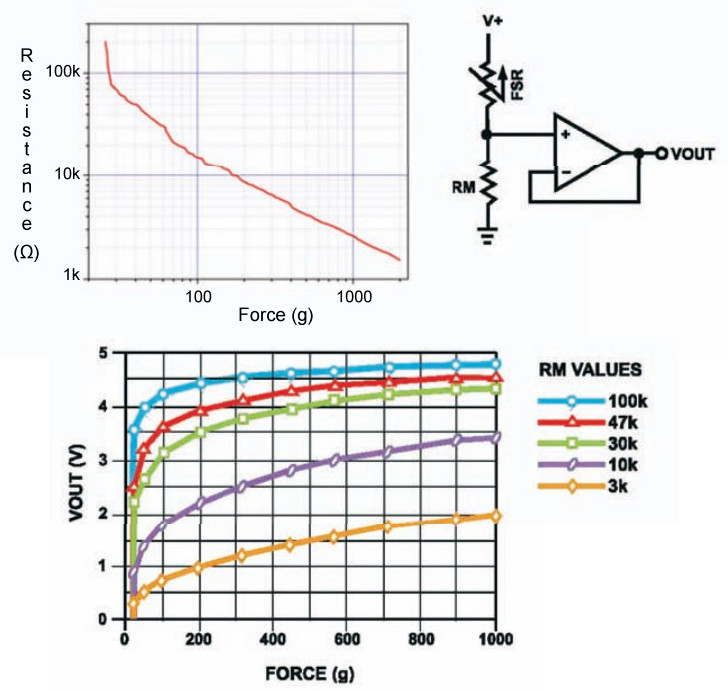
\includegraphics[width=0.6\textwidth]{./fsr-400.jpg}
\caption{Układ pomiarowy oraz wykresy zależności napięć i rezystancji od przyłożonej siły dla czujnika FSR-400}
\end{figure}

\begin{table}[h]
\centering
\begin{tabularx}
{\textwidth}{ |X|X| }
\hline
Zakres & 0,2--20 N \\
\hline
Masa & 0,15 g \\ 
\hline
Wymiary zewnętrzne & 7,6 x 7,6 x 0,4 mm \\
\hline
\end{tabularx}
\caption{Czujnik siły nacisku FSR-400}
\end{table}


\begin{table}[h]
\centering
\begin{tabularx}
{\textwidth}{ |X|X| }
\hline
Min. wartość rezystancji & 25 k$\Omega$ \\
\hline
Zakres rezystancji podczas zginania & 45--125 k$\Omega$ \\
\hline
Dł. całkowita & 73,66 mm \\
\hline
Dł. użyteczna czujnika & 55,37 mm \\ 
\hline
Szerokość & 6,35 mm \\
\hline
\end{tabularx}
\caption{Czujnik ugięcia Flex Sensor 2.2"}
\end{table}


\begin{table}[h]
\centering
\begin{tabularx}
{\textwidth}{ |X|X| }
\hline
Napięcie pracy & 2,2--3,6 V \\
\hline
Interfejs komunikacyjny & I2C \\
\hline
Rozdzielczość & 16 bitów \\
\hline
Regulowany zakres akcelerometru &  $\pm$2g, $\pm$4g, $\pm$8g, $\pm$16g \\ 
\hline
Zakres magnetometru &  od $\pm$1,3 do $\pm$8,1 gauss \\ 
\hline
Wymiary płytki & 37 x 15 mm \\
\hline
\end{tabularx}
\caption{LSM303DLHC -- 3-osiowy akcelerometr i magnetometr I2C}
\end{table}


\section{Harmonogram pracy}
\begin{enumerate}
\item (22.03.2017) Zakup elementów potrzebnych do konstrukcji \\(Krzysztof Dąbek)
\item (30.03.2017) Nawiązanie łączności płytki z komputerem (USB/Bluetooth) \\(Krzysztof Dąbek, Dymitr Choroszczak)
\item (13.04.2017) Zaprogramowanie odczytu danych z czujników (tensometrów, czujników nacisku oraz akcelerometru) \\(Anna Postawka, Krzysztof Dąbek, Dymitr Choroszczak) 
\item (27.04.2017) Montaż czujników oraz płytki na rękawicy \\(Anna Postawka)
\item (11.05.2017) Oprogramowanie wstępnego przetwarzania danych przez płytkę \\(Dymitr Choroszczak) 
\item (25.05.2017) Przygotowanie gotowej aplikacji \\(Anna Postawka, Krzysztof Dąbek, Dymitr Choroszczak)
\item (01.06.2017) Przeprowadzenie testów oraz wprowadzenie ewentualnych poprawek \\(Anna Postawka, Krzysztof Dąbek)
\item (15.06.2017) Dokumentacja projektu \\(Dymitr Choroszczak)
\end{enumerate}

\section{Schematy}
\begin{figure}[!htb]
\includegraphics[width=\textwidth]{./SchematIdeowy.png}
\caption{Schemat Ideowy}
\end{figure}
\begin{figure}[!htb]
\centering
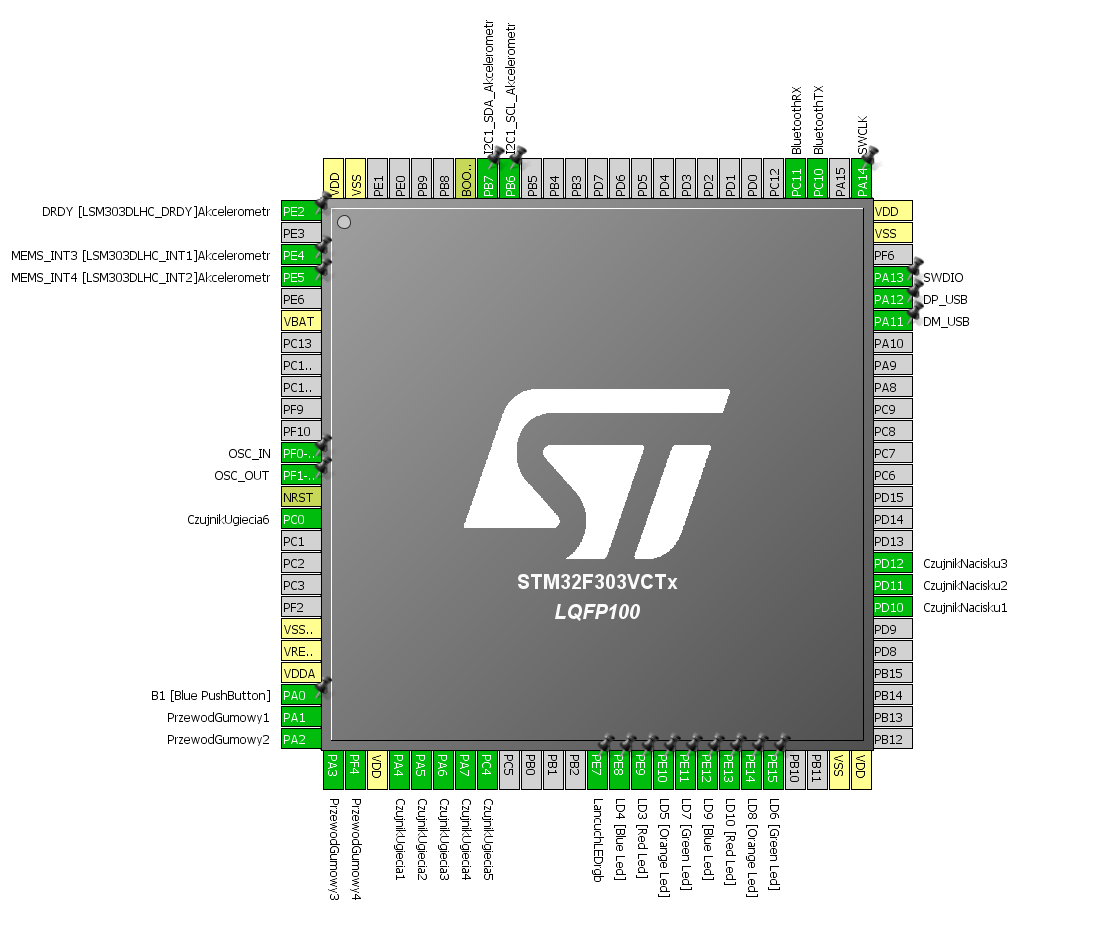
\includegraphics[width=0.6\textwidth]{./pinout.png}
\caption{Pinout dla Discovery F3}
\end{figure}
\begin{figure}[!htb]
\centering
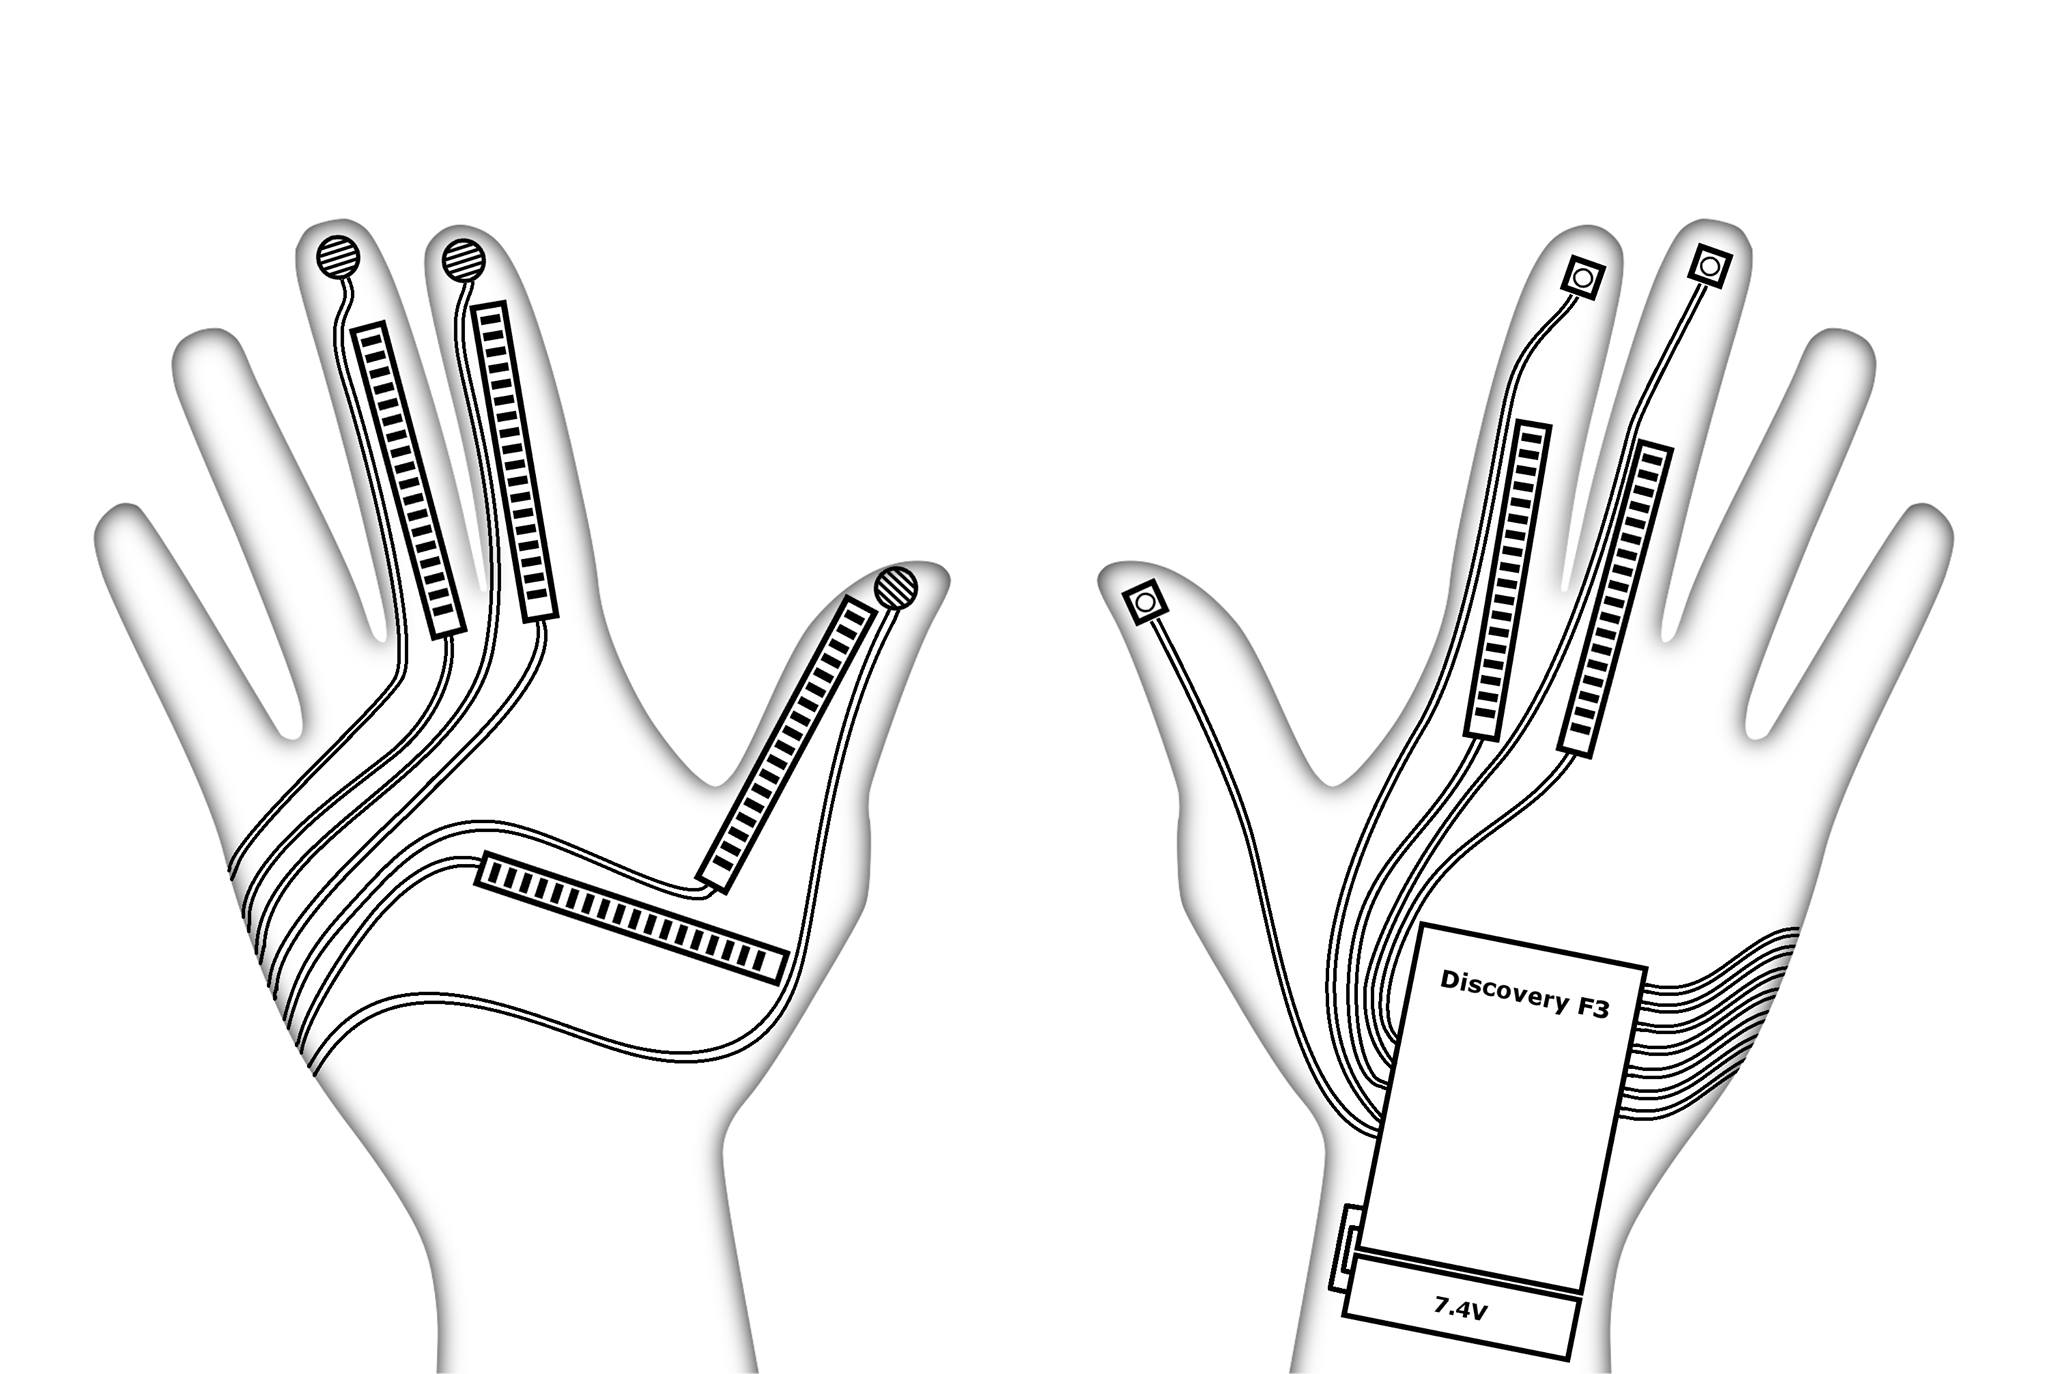
\includegraphics[width=\textwidth]{./rekawica.jpg}
\caption{Rozmieszczenie czujników na rękawicy}
\end{figure}
\end{document}
